\documentclass[conference]{IEEEtran}
\IEEEoverridecommandlockouts
\usepackage{cite}
\usepackage{amsmath,amssymb,amsfonts}
\usepackage{algorithmic}
\usepackage{algorithm}
\usepackage{graphicx}
\usepackage{textcomp}
\usepackage{xcolor}
\usepackage{booktabs}
\usepackage{multirow}
\usepackage{url}
\usepackage{hyperref}
\def\BibTeX{{\rm B\kern-.05em{\sc i\kern-.025em b}\kern-.08em
    T\kern-.1667em\lower.7ex\hbox{E}\kern-.125emX}}

\begin{document}

\title{Concept-kNN: Interpretable Graph Clustering of LLM Conversations via Classical NLP}

\author{\IEEEauthorblockN{Divyansh Bhatia}
\IEEEauthorblockA{\textit{eBay Inc.}\\
dnbhatia@ebay.com}
\and
\IEEEauthorblockN{N.~Mehala}
\IEEEauthorblockA{\textit{School of Computational and Data Sciences}\\
\textit{Vidyashilp University, Bengaluru, India}\\
mehala.n@vidyashilp.edu.in}
}

\maketitle

\begin{abstract}
Large language model (LLM) platforms generate millions of conversations spanning diverse, rapidly evolving user intents. Organizing these conversations at scale is critical for safety monitoring, misuse detection, product analytics, and emerging behavior discovery. Existing approaches rely on either lexical features (TF-IDF) or dense sentence embeddings (SBERT), paired with standard clustering algorithms. We propose Concept-kNN, a scalable, taxonomy-free clustering pipeline that uses NLP techniques---dependency parsing, named entity recognition, and noun phrase chunking---to extract sparse, interpretable concept vectors from conversation prompts, enriches them via pointwise mutual information (PMI) densification, and clusters the resulting $k$-nearest neighbor graph using Leiden community detection with a cascading singleton reassignment strategy. We evaluate on two large-scale datasets: ShareGPT (162K conversations) and LMSYS-Chat-1M (98K conversations), using LLM-generated hierarchical ground truth at three granularities (coarse, mid, fine) spanning 31--3,115 categories, validated via cross-model agreement ($\kappa \approx 0.35$, consistent across both datasets). Concept-kNN achieves a balanced NMI-coverage score of 0.627 on ShareGPT and 0.635 on LMSYS, outperforming 13 baselines---including three recent LLM-assisted methods (ClusterLLM, TnT-LLM, Clio)---by 7--21\%. A representation-algorithm ablation reveals complementary gains from concept vectors (49\%) and graph-based clustering (42\%), with a synergistic interaction: Leiden amplifies signal in concept vectors but provides negligible benefit on TF-IDF representations.
\end{abstract}

\begin{IEEEkeywords}
text clustering, conversation categorization, concept extraction, natural language processing, graph-based clustering, community detection
\end{IEEEkeywords}

% ============================================================
\section{Introduction}
% ============================================================

The rapid adoption of large language models (LLMs) has generated vast corpora of human-AI conversations spanning millions of interactions across diverse topics, languages, and user intents~\cite{zheng2024lmsys, sharegpt}. Understanding the thematic structure of these conversations is critical for content moderation, product analytics, model evaluation, and identifying emerging use patterns. However, the scale and diversity of these corpora---often containing hundreds of thousands of conversations spanning thousands of fine-grained topics---renders manual categorization infeasible and poses significant challenges for automated methods.

Traditional text clustering approaches face two fundamental limitations when applied to LLM conversations. First, \textit{representation}: lexical features (TF-IDF) capture surface-level word overlap but miss semantic similarity between topically related prompts that use different vocabulary. Dense sentence embeddings (e.g., SBERT~\cite{reimers2019sbert}) capture distributional semantics but compress information into fixed-dimensional vectors that may obscure fine-grained topical distinctions. Second, \textit{algorithm}: centroid-based methods (KMeans) require specifying the number of clusters $k$ a priori, which is unknown for real-world conversation corpora with long-tailed topic distributions. Density-based methods (HDBSCAN~\cite{campello2013hdbscan}) and topic models (BERTopic~\cite{grootendorst2022bertopic}, LDA~\cite{blei2003lda}) often leave large fractions of data unclustered or produce coarse groupings that miss fine-grained structure.

We propose \textbf{Concept-kNN}, a clustering pipeline that addresses both limitations. For representation, we apply a suite of NLP techniques---spaCy dependency parsing, named entity recognition, technical term detection, and noun phrase chunking---to extract a set of semantic \textit{concepts} from each conversation, yielding sparse, interpretable vectors whose dimensions correspond to human-readable topics. These concept vectors are enriched through PMI-based densification, which propagates topically related concepts to items that share co-occurring neighbors. For clustering, we construct a $k$-nearest neighbor similarity graph from these vectors and apply Leiden community detection~\cite{traag2019leiden}, which discovers cluster boundaries without requiring $k$ to be specified. A cascading pass-two strategy reassigns singleton nodes across six rounds at progressively relaxed similarity thresholds ($\tau$ from 0.5 to 0.0), recomputing cluster centroids after each round to maximize coverage without degrading cluster purity.

We validate LLM-generated ground truth via cross-model agreement ($\kappa \approx 0.35$, consistent across both datasets) and confirm via circular bias testing (Kendall $\tau = 1.0$, 1.8\% NMI difference) that reported advantages are independent of evaluation methodology. Our contributions are as follows:
\begin{enumerate}
    \item We introduce Concept-kNN, a scalable pipeline for fine-grained clustering of LLM conversations combining NLP-extracted concept vectors with graph-based community detection, achieving 100\% coverage without predefined category counts via cascading singleton reassignment.
    \item We propose corpus-level PMI densification that enhances neighborhood connectivity while preserving sparse, interpretable concept representations---enabling community detection to exploit topical structure without collapsing into dense embedding spaces.
    \item We demonstrate that classical NLP concept extraction matches or exceeds LLM-based alternatives, outperforming three LLM-assisted methods (ClusterLLM, TnT-LLM, Clio) by 14--21\% at zero API cost versus up to \$23 per dataset.
    \item We reveal that clustering performance critically depends on alignment between representation geometry and community detection: Leiden amplifies signal in semantic representations (+10.7\% on concepts, +14.3\% on SBERT) but degrades on lexical features ($-$0.7\% on TF-IDF), with ablation confirming complementary gains from concept vectors (49\%) and graph-based clustering (42\%).
\end{enumerate}

% ============================================================
\section{Related Work}
% ============================================================

\subsection{Text Clustering}

Classical text clustering approaches pair bag-of-words or TF-IDF representations with partitional algorithms such as KMeans~\cite{macqueen1967kmeans} or spherical KMeans~\cite{dhillon2001spherical}. These methods require specifying the number of clusters $k$ a priori, which is often unknown in exploratory settings. Hierarchical methods avoid this but scale poorly to large corpora. Topic models including LDA~\cite{blei2003lda} and NMF~\cite{lee1999nmf} discover latent themes but typically assume a moderate number of topics; even when scaled to $n\!=\!2000$, they fall well short of the thousands of fine-grained categories required in real-world conversation corpora.

More recently, neural approaches leverage pretrained language models to obtain dense embeddings. SBERT~\cite{reimers2019sbert} produces sentence-level representations that capture semantic similarity through contrastive training on natural language inference data. BERTopic~\cite{grootendorst2022bertopic} combines SBERT embeddings with UMAP dimensionality reduction~\cite{mcinnes2018umap} and HDBSCAN~\cite{campello2013hdbscan} clustering, and has become a popular choice for topic discovery. However, density-based methods often classify a large fraction of data points as noise, which is problematic when comprehensive categorization is required. UMAP's stochastic nature can also introduce instability across runs.

\subsection{Graph-Based Clustering}

Graph-based approaches construct similarity graphs and apply community detection algorithms. The Leiden algorithm~\cite{traag2019leiden} improves upon Louvain~\cite{blondel2008louvain} by guaranteeing well-connected communities and offering superior partition quality. These methods discover natural cluster boundaries without requiring the number of clusters as input, making them well-suited to corpora with unknown topic distributions. However, their performance depends critically on graph quality, which in turn depends on the underlying vector representation.

\subsection{LLM-Assisted Clustering}

A growing line of work incorporates LLMs into the clustering pipeline. ClusterLLM~\cite{zhang2023clusterllm} queries ChatGPT for triplet and pairwise judgments to fine-tune a small embedder, consistently improving cluster quality across 14 datasets at low API cost. Viswanathan et al.~\cite{viswanathan2024fewshot} show that LLMs can amplify a few expert-provided examples to guide semi-supervised clustering, enabling trade-offs between cost and accuracy. TnT-LLM~\cite{wan2024tntllm} applies a two-phase approach to Bing Copilot conversations: an LLM iteratively generates and refines a label taxonomy, then produces pseudo-labels to train lightweight classifiers at scale. Clio~\cite{tamkin2024clio} uses Claude to extract facets from millions of conversations, cluster them via embeddings and KMeans, and build hierarchical topic summaries---all while preserving user privacy. These methods achieve strong results but depend on LLM inference at clustering time, introducing cost, latency, and reproducibility constraints. Our approach instead uses classical NLP techniques---dependency parsing, named entity recognition, and noun phrase chunking---to extract concepts deterministically at negligible cost, producing comparable semantic richness without API calls.

\subsection{Conversation Analysis}

The LMSYS-Chat-1M dataset~\cite{zheng2024lmsys} includes a topic analysis using SBERT embeddings with KMeans ($k\!=\!20$). Clio~\cite{tamkin2024clio} performs large-scale conversation analysis on Claude traffic using LLM-driven facet extraction and hierarchical clustering for safety monitoring. Our work differs by targeting fine-grained unsupervised categorization at a scale two orders of magnitude beyond coarse topic discovery ($>$2,400 categories vs.\ 20 clusters), using no LLM inference at clustering time, and providing systematic comparison across 13 methods.

% ============================================================
\section{Method}
% ============================================================

The Concept-kNN pipeline consists of four stages: concept extraction, concept filtering and densification, hybrid vector construction, and graph-based clustering with cascading reassignment. Fig.~\ref{fig:pipeline} illustrates the overall architecture.

\begin{figure*}[t]
\centering
\small
\setlength{\tabcolsep}{2pt}
\begin{tabular}{c@{\hspace{2pt}}c@{\hspace{2pt}}c@{\hspace{2pt}}c@{\hspace{2pt}}c@{\hspace{2pt}}c@{\hspace{2pt}}c@{\hspace{2pt}}c}
\fbox{\parbox{1.6cm}{\centering\scriptsize\strut\textbf{Stage 1}\\\textit{NLP Extract}\\[2pt]spaCy NER,\\dep.\ parse,\\regex,\\NP chunk}} &
$\xrightarrow{\text{\tiny concepts}}$ &
\fbox{\parbox{1.6cm}{\centering\scriptsize\strut\textbf{Stage 2}\\\textit{Filter \& Weight}\\[2pt]IDF filter,\\prompt boost,\\conv.\ propagate}} &
$\xrightarrow{\text{\tiny weighted}}$ &
\fbox{\parbox{1.6cm}{\centering\scriptsize\strut\textbf{Stage 3}\\\textit{PMI Densify}\\[2pt]top-$K$ PMI\\associates\\per concept}} &
$\xrightarrow{\text{\tiny dense}}$ &
\fbox{\parbox{1.6cm}{\centering\scriptsize\strut\textbf{Stage 4}\\\textit{Hybrid Vectors}\\[2pt]$[\alpha\!\cdot\!\mathbf{v}_c;$\\$(1\!-\!\alpha)\!\cdot\!\mathbf{v}_t]$\\L2-norm}} &
$\xrightarrow{\text{\tiny vectors}}$ \\[12pt]
\multicolumn{8}{c}{
\fbox{\parbox{1.6cm}{\centering\scriptsize\strut\textbf{Stage 5}\\\textit{kNN Graph}\\[2pt]$k$=30,\\threshold $\sigma$}} \hspace{2pt}
$\xrightarrow{\text{\tiny graph}}$ \hspace{2pt}
\fbox{\parbox{1.6cm}{\centering\scriptsize\strut\textbf{Stage 6}\\\textit{Leiden}\\[2pt]community\\detection\\resolution $\gamma$}} \hspace{2pt}
$\xrightarrow{\text{\tiny labels}}$ \hspace{2pt}
\fbox{\parbox{1.6cm}{\centering\scriptsize\strut\textbf{Stage 7}\\\textit{Cascade}\\[2pt]6 rounds:\\$\tau$=0.5$\to$0.0\\reassign to\\nearest centroid}} \hspace{2pt}
$\Rightarrow$ \hspace{2pt}
\fbox{\parbox{1.6cm}{\centering\scriptsize\strut\textbf{Output}\\[2pt]\textit{100\%}\\coverage\\clusters}}
}
\end{tabular}

\vspace{4pt}
\noindent\rule{\textwidth}{0.4pt}
\vspace{2pt}

\scriptsize
\textbf{Worked example.} User prompt: \textit{``How do I fine-tune a BERT model for sentiment analysis using Hugging Face?''}\\
\textbf{Stage 1:} NER$\to$\{BERT, Hugging Face\}, dep.\ parse$\to$\{fine-tune model\}, regex$\to$\{sentiment analysis\}, NP$\to$\{BERT model\} $\Rightarrow$ 5 raw concepts\\
\textbf{Stage 2:} IDF filter retains all (df $< 8\%$); prompt boost $3\times$ $\Rightarrow$ weights: bert\,(.26), hugging face\,(.22), fine-tune model\,(.21), sentiment analysis\,(.18), bert model\,(.13)\\
\textbf{Stage 3:} PMI top-$K$ associates: ``bert'' $\to$ \{transformer, pre-trained model, tokenizer, ...\}; ``sentiment analysis'' $\to$ \{text classification, nlp, ...\} added at $0.3\times$ decay $\Rightarrow$ 12 concept dims\\
\textbf{Stage 4:} 12 concept dims $\oplus$ 5K TF-IDF dims, $\alpha\!=\!0.8$ blend, L2-norm $\Rightarrow$ one hybrid vector\\
\textbf{Stage 5--6:} kNN ($k\!=\!30$, $\sigma\!=\!0.6$) $\to$ Leiden places item in cluster whose top concepts include: \{huggingface, transformer, transfer learning, text classification, abstract class, ...\}---the GT ``programming/NLP'' cluster\\
\textbf{Stage 7:} Item already in non-singleton cluster $\to$ no reassignment needed. Nearby singleton (e.g., a rare PyTorch-Lightning question) gets assigned at $\tau\!=\!0.3$

\caption{Concept-kNN pipeline architecture with a worked example from the ShareGPT dataset. Stages 1--4 build the representation; stages 5--7 perform clustering. The cascading reassignment (Stage 7) runs 6 rounds at decreasing similarity thresholds to achieve 100\% coverage.}
\label{fig:pipeline}
\end{figure*}

\subsection{NLP Concept Extraction}

Given a conversation consisting of a user prompt $p_i$ and model response $r_i$, we extract a set of semantic concepts $C_i = \{c_1, c_2, \ldots, c_m\}$ that characterize the topical content of the interaction using a multi-stage NLP pipeline. Concepts are short phrases (1--3 words) representing topics, entities, techniques, or domains mentioned in the conversation.

The extraction pipeline proceeds as follows. First, text is cleaned by removing code blocks, URLs, file paths, and non-natural-language lines. Then, four complementary extraction strategies are applied: (1) \textit{named entity recognition} via spaCy~\cite{honnibal2020spacy} identifies proper nouns, organizations, and domain terms; (2) \textit{verb+object dependency parsing} via spaCy extracts action-oriented concept pairs (e.g., ``build website,'' ``calculate derivative'') that capture user intent; (3) \textit{technical term detection} via regex patterns identifies programming languages, frameworks, and domain-specific terminology; and (4) \textit{noun phrase chunking} captures topical multi-word expressions. Quality filters remove code artifacts, gibberish, stopwords, and overly generic terms. Concepts are extracted separately from the user prompt and the model response, enabling differential treatment of these two sources.

\subsection{Concept Filtering and Weighting}

Raw concepts undergo multi-stage filtering to remove noise:

\textbf{Name and filler removal.} Person names, LLM-generated filler phrases (e.g., ``feel free,'' ``hope this helps''), and generic single-word noise are removed using curated blocklists and regex patterns.

\textbf{IDF-based weighting.} Each surviving concept $c$ is assigned an inverse document frequency weight $\text{IDF}(c) = \log(N / \text{df}(c))$, where $N$ is the corpus size and $\text{df}(c)$ is the document frequency. Concepts with $\text{IDF}(c) < 0.5$ or document frequency outside $[3, 0.08N]$ are removed.

\textbf{Prompt boosting.} Concepts appearing in the user prompt receive a $3\times$ weight multiplier relative to response-only concepts, reflecting that user prompts are more indicative of conversational intent.

\textbf{Conversation propagation.} For multi-turn conversations, concept-sparse turns inherit concepts from the concept-richest turn in the same conversation, with an inheritance discount factor of 0.5.

\subsection{PMI Concept Densification}

Sparse concept vectors (mean 8--16 concepts per item after filtering) create connectivity challenges for graph-based clustering. To address this, we compute pairwise pointwise mutual information (PMI) between all concept pairs:
\begin{equation}
    \text{PMI}(c_i, c_j) = \log \frac{P(c_i, c_j)}{P(c_i) \cdot P(c_j)}
\end{equation}
where $P(c_i, c_j)$ is estimated from concept co-occurrence counts across items. For each concept $c$, we identify its top-$K$ associates by PMI score ($K \in \{25, 30, 35\}$, min PMI $\geq 1.0$, min concept frequency $\geq 3$). Each item then receives its concepts' associates as additional features, with weights $w_{\text{new}} = w_{\text{parent}} \cdot 0.3 \cdot \min(\text{PMI}/3, 1)$, capped at 20 new concepts per item. This densification step increases mean concepts per item from 8--16 to 20--35, improving graph connectivity without introducing topically unrelated concepts.

\subsection{Hybrid Concept-TF-IDF Vectors}

Concept vectors capture semantic topics but may miss lexical cues present in the raw text. We construct hybrid vectors by blending L2-normalized concept vectors $\mathbf{v}_c$ with TF-IDF vectors $\mathbf{v}_t$ computed from the raw prompt text (5,000 features, unigrams and bigrams, sublinear TF, English stopwords removed, same IDF frequency bounds as concept filtering):
\begin{equation}
    \mathbf{v}_{\text{hybrid}} = \text{L2-normalize}\left([\alpha \cdot \mathbf{v}_c ~;~ (1-\alpha) \cdot \mathbf{v}_t]\right)
\end{equation}
where $[~;~]$ denotes concatenation and $\alpha \in [0, 1]$ controls the blend ratio. We find $\alpha = 0.8$ consistently optimal across both datasets, indicating that concept vectors carry the primary signal while TF-IDF provides complementary lexical detail.

\subsection{Graph Construction and Community Detection}

We construct a $k$-nearest neighbor graph ($k\!=\!30$) using brute-force cosine similarity on the hybrid vectors. Edges are retained only if their cosine similarity exceeds a threshold $\sigma$ (typically 0.6), yielding a sparse graph. We symmetrize the adjacency matrix and apply the Leiden community detection algorithm~\cite{traag2019leiden} with the Reichardt--Bornholdt configuration model and resolution parameter $\gamma$ (3 iterations, seed 42) to partition the graph into communities.

\subsection{Cascading Singleton Reassignment}

Community detection typically produces a long tail of singleton clusters---items whose nearest neighbors all fall below the threshold $\sigma$, leaving them isolated in the graph. Rather than leaving these unclustered, we apply a cascading reassignment strategy over six rounds with decreasing similarity thresholds $\tau \in \{0.5, 0.4, 0.3, 0.2, 0.1, 0.0\}$. In each round: (1) we identify all current singletons (clusters of size one); (2) we compute L2-normalized centroids for every non-singleton cluster; (3) each singleton is assigned to its nearest centroid provided the cosine similarity exceeds $\tau$. Crucially, centroids are \emph{recomputed} after each round, so clusters that absorb new members shift their centroids, potentially attracting further singletons in subsequent rounds. The final round at $\tau\!=\!0.0$ serves as a catch-all, assigning every remaining singleton to its closest cluster regardless of similarity. This progressive strategy recovers singletons at successively relaxed thresholds, achieving 100\% coverage with minimal impact on cluster purity.

Algorithm~\ref{alg:pipeline} summarizes the complete Concept-kNN pipeline.

\begin{algorithm}[t]
\caption{Concept-kNN Pipeline}
\label{alg:pipeline}
\begin{algorithmic}[1]
\REQUIRE Conversations $\{(p_i, r_i)\}_{i=1}^{N}$, parameters $K$, $\alpha$, $\sigma$, $\gamma$
\ENSURE Cluster assignments $\ell \in \mathbb{Z}^N$
\STATE Extract concepts $C_i$ from each $(p_i, r_i)$ via NLP pipeline
\STATE Filter noise, compute IDF weights, apply $3\times$ prompt boost
\STATE Propagate concepts within multi-turn conversations
\STATE Compute PMI matrix; densify each $C_i$ with top-$K$ PMI associates (decay $0.3$)
\STATE Build sparse concept vectors $\mathbf{v}_c^{(i)}$, L2-normalize
\STATE Build TF-IDF vectors $\mathbf{v}_t^{(i)}$ from raw prompts ($n$-grams, sublinear TF)
\STATE $\mathbf{v}^{(i)} \leftarrow \text{normalize}([\alpha \cdot \mathbf{v}_c^{(i)} ; (1-\alpha) \cdot \mathbf{v}_t^{(i)}])$
\STATE Compute $k$-NN graph $G$ ($k\!=\!30$) with cosine similarity, threshold $\sigma$
\STATE $\ell \leftarrow \textsc{Leiden}(G, \gamma)$ \hfill \textit{\% RB config.\ model}
\FOR{$\tau \in \{0.5, 0.4, 0.3, 0.2, 0.1, 0.0\}$}
    \STATE $S \leftarrow \{i : |\{j : \ell_j = \ell_i\}| = 1\}$ \hfill \textit{\% current singletons}
    \STATE Recompute centroids $\mu_c$ for all non-singleton clusters
    \FOR{each $i \in S$}
        \STATE $c^* \leftarrow \arg\max_c \cos(\mathbf{v}^{(i)}, \mu_c)$
        \IF{$\cos(\mathbf{v}^{(i)}, \mu_{c^*}) \geq \tau$}
            \STATE $\ell_i \leftarrow c^*$
        \ENDIF
    \ENDFOR
\ENDFOR
\RETURN $\ell$
\end{algorithmic}
\end{algorithm}

% ============================================================
\section{Experimental Setup}
% ============================================================

\subsection{Datasets}

\textbf{ShareGPT}~\cite{sharegpt} contains 161,764 multi-turn conversations between users and various LLMs, collected from shared ChatGPT conversation logs. Conversations span a wide range of topics including programming, creative writing, education, and general knowledge.

\textbf{LMSYS-Chat-1M}~\cite{zheng2024lmsys} contains one million real-world conversations with 25 LLMs, collected from the Chatbot Arena platform. We sample 100,000 English-language first-turn prompts and apply a cleaning pipeline to remove system prompt contamination, template spam, and bot-generated content, yielding 97,776 clean items with 16,255 unique concepts. This dataset reflects authentic user behavior with greater topic diversity than curated alternatives.

Table~\ref{tab:datasets} summarizes the key characteristics of both datasets.

\begin{table}[t]
\caption{Dataset and ground truth characteristics after preprocessing.}
\label{tab:datasets}
\centering
\small
\begin{tabular}{@{}lcc@{}}
\toprule
\textbf{Property} & \textbf{ShareGPT} & \textbf{LMSYS} \\
\midrule
Conversations & 161,764 & 97,776 \\
Source & Shared logs & Chatbot Arena \\
Turns used & Multi-turn & First turn \\
Unique concepts & 26,561 & 16,255 \\
Mean concepts/item & 16.0 & 7.7 \\
\midrule
GT coarse categories & 35 & 31 \\
GT mid categories & 1,344 & 1,257 \\
GT fine categories & 3,115 & 2,403 \\
GT label coverage & 95.3\% & 99.7\% \\
\bottomrule
\end{tabular}
\end{table}

\subsection{Ground Truth Generation}

Since no existing fine-grained ground truth exists for these datasets at the required granularity, we generate hierarchical labels using a two-stage LLM-based annotation pipeline. In the first stage, all unique NLP-extracted concepts from the corpus are batched and sent to an LLM (GPT-5.2) for semantic categorization at three granularity levels: coarse (broad topic, e.g., ``programming''), mid-level (subcategory, e.g., ``programming:web\_development''), and fine-grained (specific topic, e.g., ``programming:web\_scraping''). Concepts are sorted by document frequency and processed in batches of 200 to provide the LLM with rich context. A caching mechanism avoids redundant API calls, and a category merge step consolidates near-duplicate subcategory names into canonical forms.

In the second stage, concept-level labels are propagated to prompts via weighted voting: each prompt inherits the category that receives the highest total weight from its constituent concepts, where weights are derived from the IDF-based concept weighting scheme (Section~3.2). This indirect approach---categorizing $\sim$16K--27K concepts rather than $\sim$98K--162K individual prompts---reduces LLM annotation cost by an order of magnitude while achieving high label coverage (95.3\%--99.7\% of prompts labeled, Table~\ref{tab:datasets}).

The resulting taxonomy contains 31--35 coarse categories, 1,257--1,344 mid-level categories, and 2,403--3,115 fine-grained categories across the two datasets (Table~\ref{tab:datasets}). Evaluation is performed at all three granularity levels to assess whether method advantages hold across different levels of categorization specificity.

\subsection{Evaluation Metric}

We evaluate clustering quality using normalized mutual information (NMI) against ground truth labels at three granularity levels: $\text{NMI}_{\text{coarse}}$, $\text{NMI}_{\text{mid}}$, and $\text{NMI}_{\text{fine}}$. For methods that may leave items unclustered (density-based and graph-based), we additionally report the \textit{balanced score}:
\begin{equation}
    \text{bal} = \text{NMI}_{\text{fine}} \times \text{coverage}
\end{equation}
where coverage is the fraction of items assigned to non-singleton clusters. This metric penalizes both poor cluster quality (low NMI) and low cluster assignment rates (low coverage), capturing the quality-coverage tradeoff inherent in density-based and graph-based methods. We use the fine-grained balanced score as the primary ranking metric, as it best captures the granularity that distinguishes methods.

\subsection{Baselines}

We compare against 13 methods spanning five representation families and multiple clustering algorithms. For all baselines, we sweep hyperparameters and report the best balanced score.

\textbf{Lexical:} TF-IDF (up to 30K features, sublinear TF) with KMeans and HDBSCAN.

\textbf{Embedding:} SBERT (\texttt{all-MiniLM-L6-v2}, 384 dim) with KMeans, HDBSCAN, Leiden, and UMAP~\cite{mcinnes2018umap} + KMeans.

\textbf{Topic models:} LDA~\cite{blei2003lda} ($n\!=\!100$), NMF~\cite{lee1999nmf} ($n \in \{100, 500, 1000, 2000\}$), BERTopic~\cite{grootendorst2022bertopic}.

\textbf{Concept-based:} Concept vectors with KMeans and Spherical KMeans~\cite{dhillon2001spherical} (ablation baselines).

\textbf{LLM-assisted:} ClusterLLM~\cite{zhang2023clusterllm} (1,024 entropy-sampled triplets fine-tune SBERT, then KMeans), TnT-LLM~\cite{wan2024tntllm} (LLM-generated taxonomy with 48K pseudo-labeled training samples for LogReg classifier), Clio~\cite{tamkin2024clio} (LLM-extracted facets embedded via SBERT, then KMeans). All use gpt-4o-mini as the LLM oracle.

KMeans variants are swept over $k \in \{5\text{K}, 10\text{K}, 15\text{K}, 20\text{K}\}$. Leiden resolution, HDBSCAN minimum cluster size, and UMAP parameters are similarly tuned.

% ============================================================
\section{Results}
% ============================================================

\subsection{Main Results}

Table~\ref{tab:main_results} presents the balanced scores across both datasets. Concept-kNN achieves the highest score on both ShareGPT (0.627) and LMSYS (0.635), outperforming the strongest non-LLM baseline (SBERT + UMAP + KMeans) by 10.4\% and 7.4\% respectively, and the strongest LLM-assisted baseline (ClusterLLM) by 17.0\% and 14.6\%.

\begin{table}[t]
\caption{Balanced scores (NMI\textsubscript{fine} $\times$ coverage) on both datasets. Best in \textbf{bold}.}
\label{tab:main_results}
\centering
\small
\begin{tabular}{@{}lcc@{}}
\toprule
\textbf{Method} & \textbf{ShareGPT} & \textbf{LMSYS} \\
\midrule
\textbf{Concept-kNN (Ours)} & \textbf{0.627} & \textbf{0.635} \\
\midrule
SBERT + UMAP + KMeans & 0.568 & 0.591 \\
SBERT + Leiden & 0.561 & 0.565 \\
Concept + KMeans & 0.555 & 0.569 \\
Spherical KMeans & 0.544 & 0.557 \\
ClusterLLM$^\dagger$ & 0.536 & 0.554 \\
Clio$^\dagger$ & 0.516 & 0.526 \\
SBERT + KMeans & 0.508 & 0.513 \\
TF-IDF + KMeans & 0.469 & 0.501 \\
\midrule
NMF (best $n$) & 0.339 & 0.340 \\
SBERT + HDBSCAN & 0.322 & 0.319 \\
BERTopic & 0.258 & 0.297 \\
TF-IDF + HDBSCAN & 0.157 & 0.197 \\
TnT-LLM$^\dagger$ & 0.131 & 0.139 \\
\bottomrule
\multicolumn{3}{@{}l}{\footnotesize $^\dagger$Requires LLM API calls at clustering time.}
\end{tabular}
\end{table}

Three performance tiers emerge consistently across both datasets. The \textit{top tier} (0.54--0.64) contains Concept-kNN and SBERT with graph-based or dimensionality-reduced clustering. The \textit{middle tier} (0.47--0.57) contains flat KMeans methods and all three LLM-assisted baselines that cluster at fine granularity; notably, neither ClusterLLM's LLM-guided fine-tuning nor Clio's LLM-extracted facets surpass SBERT+UMAP+KMeans. The \textit{bottom tier} ($<$0.34) contains density-based methods, topic models, and TnT-LLM, whose taxonomy-then-classify design produces only 58--64 effective clusters---far too coarse for fine-grained evaluation against 2,403--3,115 ground truth categories.

The LLM-assisted baselines are informative. ClusterLLM uses 1,024 LLM triplet judgments to fine-tune SBERT, gaining +0.03--0.04 over vanilla SBERT+KMeans---but still falling below SBERT+UMAP+KMeans. Clio replaces NLP extraction with LLM-generated facets: each prompt is sent to gpt-4o-mini, facets are embedded via SBERT, and KMeans clusters the result. Despite \$23 in API costs and 86 hours of facet extraction across both datasets, Clio (0.516/0.526) underperforms Concept-kNN (0.627/0.635) by 21\% and 21\% respectively. Concept-kNN's NLP-extracted concepts capture comparable semantic signal at zero cost. TnT-LLM faces a more fundamental challenge: its taxonomy-then-classify design produces only 58--64 effective clusters from $\sim$97--98 LLM-generated categories, yielding 0.131 on ShareGPT and 0.139 on LMSYS despite requiring 10+ hours of LLM inference per dataset.

\subsection{Cross-Dataset Consistency}

The consistency across datasets is notable. Despite substantial differences---ShareGPT contains curated multi-turn conversations while LMSYS contains raw single-turn queries; concept density differs (16 vs.\ 7.7 per item)---all methods maintain the same relative ranking and optimal hyperparameters transfer ($\alpha\!=\!0.8$, $\sigma\!=\!0.6$, PMI $K\!=\!35$), with only resolution $\gamma$ differing (80 vs.\ 50).

\subsection{Multi-Granularity Analysis}

To assess whether Concept-kNN's advantage holds across different levels of categorization specificity, we evaluate NMI at all three ground truth granularity levels. Table~\ref{tab:multigran} presents results for selected methods on both datasets.

\begin{table}[t]
\caption{NMI at three granularity levels. Top section: full-coverage methods (ranked by bal). Bottom section: partial-coverage methods. Best raw NMI per column in \underline{underline}.}
\label{tab:multigran}
\centering
\small
\setlength{\tabcolsep}{3.5pt}
\begin{tabular}{@{}l ccc ccc@{}}
\toprule
& \multicolumn{3}{c}{\textbf{ShareGPT}} & \multicolumn{3}{c}{\textbf{LMSYS}} \\
\cmidrule(lr){2-4}\cmidrule(lr){5-7}
\textbf{Method} & \textbf{C} & \textbf{M} & \textbf{F} & \textbf{C} & \textbf{M} & \textbf{F} \\
\midrule
\textbf{Concept-kNN} & \textbf{.280} & \textbf{.541} & \textbf{.627} & \textbf{.316} & \textbf{.574} & \textbf{.635} \\
SBERT+UMAP+KM & .239 & .484 & .570 & .287 & .539 & .597 \\
SBERT+Leiden & .237 & .477 & .561 & .268 & .507 & .565 \\
Sph.\ KMeans & .232 & .466 & .550 & .278 & .519 & .577 \\
TF-IDF+KMeans & .174 & .389 & .475 & .225 & .452 & .512 \\
\midrule
TF-IDF+HDBSCAN & \underline{.320} & \underline{.559} & \underline{.633} & \underline{.354} & \underline{.587} & \underline{.639} \\
BERTopic & .319 & .537 & .603 & .343 & .564 & .614 \\
SBERT+HDBSCAN & .307 & .544 & .620 & .340 & .572 & .625 \\
\bottomrule
\end{tabular}
\end{table}

The multi-granularity results reveal two findings. First, density-based methods achieve the highest \textit{raw} NMI at every granularity---TF-IDF+HDBSCAN reaches 0.639 on LMSYS fine---but their coverage (25--51\%) makes them impractical. Second, among full-coverage methods, Concept-kNN's advantage \textit{widens} at finer granularity: on ShareGPT, the gap versus SBERT+UMAP+KMeans grows from +0.041 (coarse) to +0.057 (fine), suggesting concept representations are particularly effective at fine-grained distinctions that embeddings compress away.

\subsection{NMI--Coverage Decomposition}

Table~\ref{tab:component} decomposes the balanced score into NMI and coverage on ShareGPT.

\begin{table}[t]
\caption{Decomposition of balanced score into NMI and coverage on ShareGPT for selected methods.}
\label{tab:component}
\centering
\small
\begin{tabular}{@{}lccc@{}}
\toprule
\textbf{Method} & \textbf{NMI\textsubscript{fine}} & \textbf{Coverage} & \textbf{Balanced} \\
\midrule
Concept-kNN (Ours) & 0.627 & 100\% & \textbf{0.627} \\
SBERT + UMAP + KMeans & 0.570 & 99.8\% & 0.568 \\
SBERT + Leiden & 0.561 & 100\% & 0.561 \\
Concept + KMeans & 0.555 & 100\% & 0.555 \\
TF-IDF + KMeans & 0.475 & 98.8\% & 0.469 \\
BERTopic & 0.603 & 42.8\% & 0.258 \\
SBERT + HDBSCAN & 0.620 & 51.8\% & 0.322 \\
TF-IDF + HDBSCAN & 0.633 & 24.8\% & 0.157 \\
\bottomrule
\end{tabular}
\end{table}

KMeans-based methods achieve near-complete coverage, so their balanced score approximately equals NMI. Density-based methods achieve \textit{higher} raw NMI on their clustered subset (TF-IDF+HDBSCAN: 0.633) but low coverage (25--52\%) penalizes the balanced score. Leiden pre-cascade achieves NMI\textsubscript{fine} of 0.670 at 74\% coverage (Table~\ref{tab:cascade}); the cascade trades 6\% NMI for full coverage.

\subsection{Qualitative Examples}

Table~\ref{tab:cluster_examples} illustrates the interpretability of discovered clusters. The Java cluster ($n\!=\!276$, 80\% purity) surfaces framework-specific concepts, the Genshin Impact cluster captures game entity names, and the Fiction cluster groups prompts around a single user's invented universe via proper nouns appearing nowhere else in the corpus.

Not all clusters are coherent: one cluster ($n\!=\!150$, 31\% purity) dominated by the generic concept ``best way'' groups unrelated queries, illustrating that high-frequency verb+object phrases can create spurious bridges.

% ============================================================
\section{Ablation Study}
% ============================================================

To understand the relative contribution of each component, we conduct a representation $\times$ algorithm ablation on the ShareGPT dataset. Table~\ref{tab:ablation} presents the complete $3 \times 2$ matrix plus the hybrid extension.

\begin{table}[t]
\caption{Representation $\times$ Algorithm ablation on ShareGPT. Each cell shows the best balanced score for that combination.}
\label{tab:ablation}
\centering
\small
\begin{tabular}{@{}lccc@{}}
\toprule
\textbf{Representation} & \textbf{KMeans} & \textbf{Leiden} & \textbf{Algo.\ $\Delta$} \\
\midrule
TF-IDF (30K dim) & 0.487 & 0.484 & $-$0.7\% \\
SBERT (384 dim) & 0.491 & 0.561 & +14.3\% \\
Concepts (PMI=35) & 0.555 & 0.615 & +10.7\% \\
\midrule
+ Hybrid $\alpha\!=\!0.8$ & --- & \textbf{0.627} & --- \\
\bottomrule
\end{tabular}
\end{table}

\subsection{Contribution Decomposition}

Starting from the TF-IDF + KMeans baseline (0.487), the total improvement to Concept-kNN (0.627) is +0.140 (+28.7\%), decomposing into: \textbf{concept representation} (+0.068, 49\%): replacing TF-IDF with concept vectors improves from 0.487 to 0.555, also outperforming SBERT (0.491 under KMeans); \textbf{graph-based clustering} (+0.059, 42\%): Leiden with cascading improves from 0.555 to 0.615; and \textbf{hybrid blending} (+0.013, 9\%): adding TF-IDF at $\alpha\!=\!0.8$ provides a modest boost to 0.627.

\subsection{Cascade Mechanism Analysis}

Table~\ref{tab:cascade} traces performance through each cascade round. Leiden alone achieves high NMI (0.670/0.671) but leaves 26\%/22\% of items as singletons. Each successive round reassigns singletons to their nearest cluster centroid at progressively relaxed thresholds, trading a small NMI decrease for a large coverage increase.

\begin{table}[t]
\caption{Cascade round-by-round on both datasets. $\tau$: similarity threshold; Asgn: items assigned in that round. NMI decreases modestly ($-$6\%) while coverage rises from $\sim$75\% to 100\%, yielding monotonically increasing bal at every round.}
\label{tab:cascade}
\centering
\footnotesize
\setlength{\tabcolsep}{2.5pt}
\begin{tabular}{@{}l r rr rr@{}}
\toprule
& & \multicolumn{2}{c}{\textbf{ShareGPT}} & \multicolumn{2}{c}{\textbf{LMSYS}} \\
\cmidrule(lr){3-4} \cmidrule(lr){5-6}
\textbf{Stage} & $\boldsymbol{\tau}$ & \textbf{Cov\%} & \textbf{Bal} & \textbf{Cov\%} & \textbf{Bal} \\
\midrule
Leiden & --- & 73.9 & .495 & 78.5 & .526 \\
Round 1 & 0.5 & 81.7 & .538 & 86.4 & .569 \\
Round 2 & 0.4 & 86.6 & .563 & 90.2 & .589 \\
Round 3 & 0.3 & 91.3 & .587 & 94.0 & .608 \\
Round 4 & 0.2 & 97.9 & .617 & 99.3 & .632 \\
Round 5 & 0.1 & 99.8 & .625 & 100.0 & .635 \\
Round 6 & 0.0 & 100.0 & .626 & 100.0 & .635 \\
\midrule
\multicolumn{2}{@{}l}{NMI\textsubscript{fine} drop} & \multicolumn{2}{c}{.670 $\to$ .626 ($-$6.5\%)} & \multicolumn{2}{c}{.671 $\to$ .635 ($-$5.3\%)} \\
\bottomrule
\end{tabular}
\end{table}

The coverage--NMI trade-off is highly favorable: a 5--7\% NMI decrease purchases a 22--26 percentage-point coverage increase, yielding \textit{monotonically increasing} balanced scores at every round. Recomputing centroids between rounds prevents early misassignments from compounding. Round~4 ($\tau\!=\!0.2$) is the pivotal step, reassigning 25\% of all singletons as the relaxed threshold catches items with moderate but genuine similarity. The final two rounds ($\tau \leq 0.1$) contribute minimally.

\subsection{Synergistic Interaction Effect}

The most notable finding is the \textit{interaction} between representation and algorithm. Leiden provides dramatically different gains depending on representation: $-$0.7\% on TF-IDF, +14.3\% on SBERT, +10.7\% on concepts. This arises because Leiden relies on modular graph structure---sparse TF-IDF vectors produce noisy kNN graphs, while semantic representations produce denser, more modular graphs with clear inter-cluster gaps.

% ============================================================
\section{Hyperparameter Analysis}
% ============================================================

We analyze hyperparameter sensitivity across 324 configurations on ShareGPT and 252 on LMSYS. Table~\ref{tab:hyperparams} summarizes the optimal values and Fig.~\ref{fig:sensitivity} visualizes the sensitivity trends.

\begin{table}[t]
\caption{Optimal hyperparameters across datasets.}
\label{tab:hyperparams}
\centering
\small
\begin{tabular}{@{}lccc@{}}
\toprule
\textbf{Parameter} & \textbf{ShareGPT} & \textbf{LMSYS} & \textbf{Transfers?} \\
\midrule
Blend $\alpha$ & 0.80 & 0.80 & Yes \\
Threshold $\sigma$ & 0.60 & 0.60 & Yes \\
PMI top-$K$ & 35 & 35 & Yes \\
Resolution $\gamma$ & 80 & 50 & Approx. \\
\bottomrule
\end{tabular}
\end{table}

\begin{figure}[t]
\centering
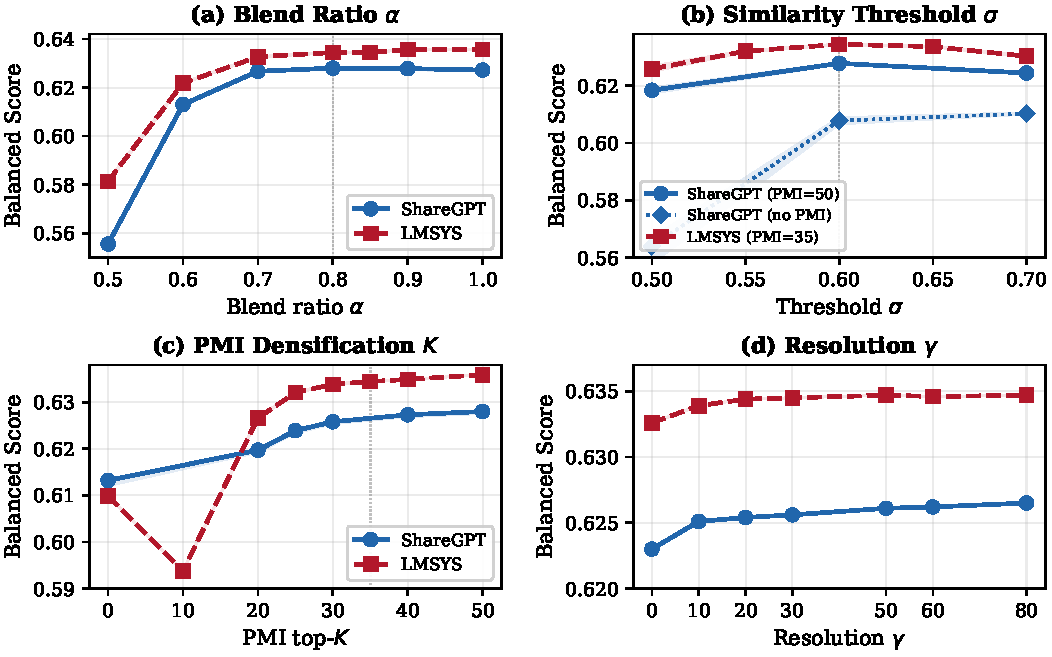
\includegraphics[width=\columnwidth]{hyperparam_sensitivity.pdf}
\caption{Hyperparameter sensitivity on both datasets. Shaded bands show variation across non-swept parameters. (a)~$\alpha$ has the strongest effect: steep climb to 0.8, then plateau through 1.0. (b)~$\sigma$ peaks at 0.6 with PMI; without PMI (dotted), sparser vectors prefer $\sigma\!=\!0.7$. (c)~PMI-$K$ shows a dip at $K\!=\!10$ on LMSYS (insufficient densification creates noisy bridges) before recovery and plateau above $K\!=\!25$. (d)~Resolution $\gamma$ shows a modest but consistent gain from $\gamma\!=\!0$ to $\gamma\!=\!30$, confirming that Leiden community detection does contribute beyond the cascading reassignment alone.}
\label{fig:sensitivity}
\end{figure}

Fig.~\ref{fig:sensitivity} reveals a clear hierarchy: $\alpha$ has the strongest effect (panel a), $\sigma$ peaks sharply at 0.6 (panel b), PMI-$K$ plateaus above 30 (panel c), and resolution $\gamma$ has minimal effect (panel d). The top-7 configurations score within 0.002 of the best.

% ============================================================
\section{Discussion}
% ============================================================

\subsection{Interpretability}

A practical advantage of concept-based representations is interpretability. Each cluster is described by its highest-weight concepts, yielding human-readable topic labels (Table~\ref{tab:cluster_examples}), unlike SBERT-based clusters requiring separate interpretation. This enables content moderation teams to monitor emerging topics without manual review.

\begin{table}[t]
\centering
\caption{Example clusters discovered by Concept-kNN on ShareGPT, showing top concepts, a representative prompt, and coarse purity (fraction sharing the dominant GT label).}
\label{tab:cluster_examples}
\footnotesize
\setlength{\tabcolsep}{2pt}
\begin{tabular}{p{1.1cm}p{2.4cm}p{3.0cm}r}
\toprule
\textbf{Cluster} & \textbf{Top Concepts} & \textbf{Example Prompt} & \textbf{Pur.} \\
\midrule
Java \newline{\scriptsize(n=276)} & java, maven, spring mvc, spring boot & ``If I am going to use Java, could you suggest me a complete technology stack?'' & .80 \\[2pt]
Genshin \newline{\scriptsize(n=138)} & liyue, beidou, klee, mondstadt, genshin impact, ningguang & ``Provide me extremely detailed steps in UE5 to create a combat system like Genshin Impact'' & .51 \\[2pt]
Fiction \newline{\scriptsize(n=129)} & jaedala, prince wukong, parvati, luxian empire, golden eyes, empress & ``I need help developing a calendar that the Luxian Empire might use.'' & .67 \\
\bottomrule
\end{tabular}
\end{table}

\subsection{Computational Cost and Complexity}

Table~\ref{tab:runtime} reports wall-clock times on LMSYS (98K, CPU). Concept-kNN completes in $\sim$200s---6$\times$ faster than SBERT+UMAP+KMeans and 48$\times$ faster than Concept+KMeans---due to sparse kNN search and Leiden's avoidance of $O(nk)$ KMeans iterations. LLM-assisted baselines incur additional API costs: Clio $\sim$\$9 and 33 hours on LMSYS; TnT-LLM $\sim$\$3.50.

\begin{table}[t]
\caption{Clustering runtime on LMSYS (98K, CPU only). Excludes one-time extraction/embedding.}
\label{tab:runtime}
\centering
\footnotesize
\begin{tabular}{@{}lrrr@{}}
\toprule
\textbf{Method} & \textbf{Time (s)} & \textbf{Bal.} & \textbf{Slowdown} \\
\midrule
Concept-kNN (Ours) & 200 & \textbf{.636} & 1$\times$ \\
SBERT + Leiden & 960 & .565 & 5$\times$ \\
SBERT + UMAP + KMeans & 1,245 & .591 & 6$\times$ \\
Spherical KMeans & 5,612 & .557 & 28$\times$ \\
SBERT + KMeans & 3,467 & .513 & 17$\times$ \\
Concept + KMeans & 9,693 & .569 & 48$\times$ \\
\bottomrule
\end{tabular}
\end{table}

Per-stage complexities: concept extraction $O(NL)$; PMI $O(V^2)$; kNN graph $O(N^2 d)$ brute-force; Leiden $O(N + E)$ per iteration~\cite{traag2019leiden}; cascade $O(RSC)$ for $R{=}6$ rounds, $S$ singletons, $C$ clusters. The bottleneck is kNN construction, reducible to $O(Nd\log N)$ via approximate nearest neighbor libraries (FAISS, Annoy).

\subsection{Ground Truth Validation}

Since GT is LLM-generated (Section~4.2), we validate via the LLM-as-a-judge paradigm~\cite{zheng2024judge, gilardi2023chatgpt}. An independent LLM (Claude Opus~4.5) re-categorizes 1,000 stratified prompts per dataset into 29 coarse categories, yielding Cohen's $\kappa = 0.347$ on ShareGPT and $\kappa = 0.344$ on LMSYS~\cite{landis1977kappa} with acceptance rates of 58.8\% and 55.1\%. The moderate $\kappa$ reflects systematic boundary ambiguity: the \textit{technology}~$\leftrightarrow$~\textit{programming} boundary accounts for 23\% of disagreements, while unambiguous categories achieve near-perfect acceptance (programming 92\%, gaming 100\%).

To test for circular bias, we used the judge's independent labels as concept-free alternative GT and recomputed NMI\textsubscript{coarse} for six methods on 995 shared prompts. Rankings were perfectly preserved (Kendall $\tau = 1.0$): Concept-kNN ranked first under both GTs. The NMI ratio averaged 1.038 for concept-based methods versus 1.020 for embedding-based---a 1.8\% difference confirming Concept-kNN's advantage is not an artifact of concept-based evaluation.

To further validate, three independent human annotators categorized 100 stratified prompts (50 per dataset) into the same 29 categories. Inter-annotator agreement averaged $\kappa = 0.81$ [0.69, 0.95] with 75\% unanimous and 100\% majority agreement, substantially exceeding the LLM cross-model $\kappa \approx 0.35$. This confirms the moderate LLM $\kappa$ reflects concept-to-prompt propagation ambiguity rather than inherent category confusion; the categories are well-defined, and the GT is noisy but unbiased.

\subsection{Design Choices and Broader Implications}

Pipeline heuristics were selected empirically but are not brittle: bal varies by $<$1\% for $\alpha \in [0.7, 1.0]$, $\sigma \in [0.55, 0.70]$, $\gamma \in [20, 80]$. PMI $\geq 1.0$ ensures associations at least twice as likely as chance. Cross-dataset consistency provides evidence of domain robustness. Concept-kNN demonstrates that classical NLP remains competitive with LLM-based approaches, with practical value for reproducible, cost-free conversation monitoring.

\subsection{Limitations}

The NLP pipeline relies on spaCy's English \texttt{en\_core\_web\_sm} model, limiting portability to other languages; larger models may improve extraction quality at additional cost. Generic verb+object phrases (e.g., ``best way'') can form spurious clusters. Performance on domain-specific corpora (e.g., medical, legal) remains untested.

% ============================================================
\section{Conclusion}
% ============================================================

We presented Concept-kNN, a conversation clustering pipeline combining NLP-extracted concept vectors with graph-based community detection. On ShareGPT (162K) and LMSYS-Chat-1M (98K), it outperforms 13 baselines---including three LLM-assisted methods---by 7--21\%. Ablation reveals complementary gains from concept representations (49\%) and Leiden clustering (42\%), with graph-based detection amplifying signal in semantic but not lexical representations. Cross-model validation ($\kappa \approx 0.35$), circular bias testing ($\tau = 1.0$), and human annotation ($\kappa = 0.81$) confirm evaluation independence. By relying on classical NLP, the pipeline is reproducible, cost-free, and scalable. Future work includes multilingual extension, multi-turn context integration, and direct prompt-level annotation.

\section*{Reproducibility}

All experiments ran on a single machine with an NVIDIA A100 GPU (concept extraction and clustering on CPU; SBERT encoding on GPU). Software: Python 3.10, spaCy 3.8.11 (\texttt{en\_core\_web\_sm} 3.8.0), scikit-learn 1.7.2, Sentence-Transformers 3.3.0 (\texttt{all-MiniLM-L6-v2}), PyTorch 2.1.0 (CUDA 12.1), igraph 1.0.0, leidenalg 0.11.0. Leiden: 3 iterations, seed 42. Concept extraction: $\sim$3\,h\,15\,m (ShareGPT), $\sim$3\,h\,54\,m (LMSYS); clustering: $\sim$200\,s per dataset. Code will be released upon publication.

\noindent\textbf{Acknowledgment.} We thank the creators of the ShareGPT and LMSYS-Chat-1M datasets for making their data publicly available.

\begin{thebibliography}{00}

\bibitem{zheng2024lmsys}
L. Zheng, W.-L. Chiang, Y. Sheng, S. Zhuang, Z. Wu, Y. Zhuang, Z. Lin, Z. Li, D. Li, E. Xing, H. Zhang, J. E. Gonzalez, and I. Stoica, ``LMSYS-Chat-1M: A large-scale real-world LLM conversation dataset,'' in \textit{Proc. ICLR}, 2024.

\bibitem{sharegpt}
ShareGPT, ``ShareGPT: Share your ChatGPT conversations,'' 2023. [Online]. Available: \url{https://sharegpt.com}

\bibitem{reimers2019sbert}
N. Reimers and I. Gurevych, ``Sentence-BERT: Sentence embeddings using Siamese BERT-networks,'' in \textit{Proc. EMNLP-IJCNLP}, 2019, pp. 3982--3992.

\bibitem{campello2013hdbscan}
R. J. G. B. Campello, D. Moulavi, and J. Sander, ``Density-based clustering based on hierarchical density estimates,'' in \textit{Proc. PAKDD}, 2013, pp. 160--172.

\bibitem{grootendorst2022bertopic}
M. Grootendorst, ``BERTopic: Neural topic modeling with a class-based TF-IDF procedure,'' 2022. [Online]. Available: \url{https://arxiv.org/abs/2203.05794}

\bibitem{blei2003lda}
D. M. Blei, A. Y. Ng, and M. I. Jordan, ``Latent Dirichlet allocation,'' \textit{J. Mach. Learn. Res.}, vol. 3, pp. 993--1022, 2003.

\bibitem{traag2019leiden}
V. A. Traag, L. Waltman, and N. J. van Eck, ``From Louvain to Leiden: Guaranteeing well-connected communities,'' \textit{Sci. Rep.}, vol. 9, no. 1, p. 5233, 2019.

\bibitem{blondel2008louvain}
V. D. Blondel, J.-L. Guillaume, R. Lambiotte, and E. Lefebvre, ``Fast unfolding of communities in large networks,'' \textit{J. Stat. Mech.}, vol. 2008, no. 10, p. P10008, 2008.

\bibitem{macqueen1967kmeans}
J. MacQueen, ``Some methods for classification and analysis of multivariate observations,'' in \textit{Proc. 5th Berkeley Symp. Math. Stat. Probab.}, vol. 1, 1967, pp. 281--297.

\bibitem{dhillon2001spherical}
I. S. Dhillon and D. S. Modha, ``Concept decompositions for large sparse text data using clustering,'' \textit{Mach. Learn.}, vol. 42, pp. 143--175, 2001.

\bibitem{lee1999nmf}
D. D. Lee and H. S. Seung, ``Learning the parts of objects by non-negative matrix factorization,'' \textit{Nature}, vol. 401, pp. 788--791, 1999.

\bibitem{zhang2023clusterllm}
Y. Zhang, Z. Wang, and J. Shang, ``ClusterLLM: Large language models as a guide for text clustering,'' in \textit{Proc. EMNLP}, 2023, pp. 13903--13920.

\bibitem{viswanathan2024fewshot}
V. Viswanathan, K. Gashteovski, C. Lawrence, T. Wu, and G. Neubig, ``Large language models enable few-shot clustering,'' \textit{Trans. Assoc. Comput. Linguist.}, vol. 12, pp. 321--333, 2024.

\bibitem{wan2024tntllm}
M. Wan, et al., ``TnT-LLM: Text mining at scale with large language models,'' in \textit{Proc. KDD}, 2024, pp. 6160--6171.

\bibitem{tamkin2024clio}
A. Tamkin, et al., ``Clio: Privacy-preserving insights into real-world AI use,'' \textit{arXiv:2412.13678}, 2024.

\bibitem{mcinnes2018umap}
L. McInnes, J. Healy, and J. Melville, ``UMAP: Uniform manifold approximation and projection for dimension reduction,'' 2018. [Online]. Available: \url{https://arxiv.org/abs/1802.03426}

\bibitem{honnibal2020spacy}
M. Honnibal, I. Montani, S. Van Landeghem, and A. Boyd, ``spaCy: Industrial-strength natural language processing in Python,'' 2020. [Online]. Available: \url{https://spacy.io}

\bibitem{gilardi2023chatgpt}
F. Gilardi, M. Alizadeh, and M. Kubli, ``ChatGPT outperforms crowd-workers for text-annotation tasks,'' \textit{Proc. Natl. Acad. Sci.}, vol. 120, no. 30, e2305016120, 2023.

\bibitem{zheng2024judge}
L. Zheng, W.-L. Chiang, Y. Sheng, S. Zhuang, Z. Wu, Y. Zhuang, Z. Lin, Z. Li, D. Li, E. Xing, H. Zhang, J. E. Gonzalez, and I. Stoica, ``Judging LLM-as-a-judge with MT-Bench and Chatbot Arena,'' in \textit{Proc. NeurIPS}, 2023.

\bibitem{landis1977kappa}
J. R. Landis and G. G. Koch, ``The measurement of observer agreement for categorical data,'' \textit{Biometrics}, vol. 33, no. 1, pp. 159--174, 1977.

\end{thebibliography}

\end{document}